
% Default to the notebook output style

    


% Inherit from the specified cell style.




    
\documentclass[11pt]{article}

    
    
    \usepackage[T1]{fontenc}
    % Nicer default font (+ math font) than Computer Modern for most use cases
    \usepackage{mathpazo}

    % Basic figure setup, for now with no caption control since it's done
    % automatically by Pandoc (which extracts ![](path) syntax from Markdown).
    \usepackage{graphicx}
    % We will generate all images so they have a width \maxwidth. This means
    % that they will get their normal width if they fit onto the page, but
    % are scaled down if they would overflow the margins.
    \makeatletter
    \def\maxwidth{\ifdim\Gin@nat@width>\linewidth\linewidth
    \else\Gin@nat@width\fi}
    \makeatother
    \let\Oldincludegraphics\includegraphics
    % Set max figure width to be 80% of text width, for now hardcoded.
    \renewcommand{\includegraphics}[1]{\Oldincludegraphics[width=.8\maxwidth]{#1}}
    % Ensure that by default, figures have no caption (until we provide a
    % proper Figure object with a Caption API and a way to capture that
    % in the conversion process - todo).
    \usepackage{caption}
    \DeclareCaptionLabelFormat{nolabel}{}
    \captionsetup{labelformat=nolabel}

    \usepackage{adjustbox} % Used to constrain images to a maximum size 
    \usepackage{xcolor} % Allow colors to be defined
    \usepackage{enumerate} % Needed for markdown enumerations to work
    \usepackage{geometry} % Used to adjust the document margins
    \usepackage{amsmath} % Equations
    \usepackage{amssymb} % Equations
    \usepackage{textcomp} % defines textquotesingle
    % Hack from http://tex.stackexchange.com/a/47451/13684:
    \AtBeginDocument{%
        \def\PYZsq{\textquotesingle}% Upright quotes in Pygmentized code
    }
    \usepackage{upquote} % Upright quotes for verbatim code
    \usepackage{eurosym} % defines \euro
    \usepackage[mathletters]{ucs} % Extended unicode (utf-8) support
    \usepackage[utf8x]{inputenc} % Allow utf-8 characters in the tex document
    \usepackage{fancyvrb} % verbatim replacement that allows latex
    \usepackage{grffile} % extends the file name processing of package graphics 
                         % to support a larger range 
    % The hyperref package gives us a pdf with properly built
    % internal navigation ('pdf bookmarks' for the table of contents,
    % internal cross-reference links, web links for URLs, etc.)
    \usepackage{hyperref}
    \usepackage{longtable} % longtable support required by pandoc >1.10
    \usepackage{booktabs}  % table support for pandoc > 1.12.2
    \usepackage[inline]{enumitem} % IRkernel/repr support (it uses the enumerate* environment)
    \usepackage[normalem]{ulem} % ulem is needed to support strikethroughs (\sout)
                                % normalem makes italics be italics, not underlines
    

    
    
    % Colors for the hyperref package
    \definecolor{urlcolor}{rgb}{0,.145,.698}
    \definecolor{linkcolor}{rgb}{.71,0.21,0.01}
    \definecolor{citecolor}{rgb}{.12,.54,.11}

    % ANSI colors
    \definecolor{ansi-black}{HTML}{3E424D}
    \definecolor{ansi-black-intense}{HTML}{282C36}
    \definecolor{ansi-red}{HTML}{E75C58}
    \definecolor{ansi-red-intense}{HTML}{B22B31}
    \definecolor{ansi-green}{HTML}{00A250}
    \definecolor{ansi-green-intense}{HTML}{007427}
    \definecolor{ansi-yellow}{HTML}{DDB62B}
    \definecolor{ansi-yellow-intense}{HTML}{B27D12}
    \definecolor{ansi-blue}{HTML}{208FFB}
    \definecolor{ansi-blue-intense}{HTML}{0065CA}
    \definecolor{ansi-magenta}{HTML}{D160C4}
    \definecolor{ansi-magenta-intense}{HTML}{A03196}
    \definecolor{ansi-cyan}{HTML}{60C6C8}
    \definecolor{ansi-cyan-intense}{HTML}{258F8F}
    \definecolor{ansi-white}{HTML}{C5C1B4}
    \definecolor{ansi-white-intense}{HTML}{A1A6B2}

    % commands and environments needed by pandoc snippets
    % extracted from the output of `pandoc -s`
    \providecommand{\tightlist}{%
      \setlength{\itemsep}{0pt}\setlength{\parskip}{0pt}}
    \DefineVerbatimEnvironment{Highlighting}{Verbatim}{commandchars=\\\{\}}
    % Add ',fontsize=\small' for more characters per line
    \newenvironment{Shaded}{}{}
    \newcommand{\KeywordTok}[1]{\textcolor[rgb]{0.00,0.44,0.13}{\textbf{{#1}}}}
    \newcommand{\DataTypeTok}[1]{\textcolor[rgb]{0.56,0.13,0.00}{{#1}}}
    \newcommand{\DecValTok}[1]{\textcolor[rgb]{0.25,0.63,0.44}{{#1}}}
    \newcommand{\BaseNTok}[1]{\textcolor[rgb]{0.25,0.63,0.44}{{#1}}}
    \newcommand{\FloatTok}[1]{\textcolor[rgb]{0.25,0.63,0.44}{{#1}}}
    \newcommand{\CharTok}[1]{\textcolor[rgb]{0.25,0.44,0.63}{{#1}}}
    \newcommand{\StringTok}[1]{\textcolor[rgb]{0.25,0.44,0.63}{{#1}}}
    \newcommand{\CommentTok}[1]{\textcolor[rgb]{0.38,0.63,0.69}{\textit{{#1}}}}
    \newcommand{\OtherTok}[1]{\textcolor[rgb]{0.00,0.44,0.13}{{#1}}}
    \newcommand{\AlertTok}[1]{\textcolor[rgb]{1.00,0.00,0.00}{\textbf{{#1}}}}
    \newcommand{\FunctionTok}[1]{\textcolor[rgb]{0.02,0.16,0.49}{{#1}}}
    \newcommand{\RegionMarkerTok}[1]{{#1}}
    \newcommand{\ErrorTok}[1]{\textcolor[rgb]{1.00,0.00,0.00}{\textbf{{#1}}}}
    \newcommand{\NormalTok}[1]{{#1}}
    
    % Additional commands for more recent versions of Pandoc
    \newcommand{\ConstantTok}[1]{\textcolor[rgb]{0.53,0.00,0.00}{{#1}}}
    \newcommand{\SpecialCharTok}[1]{\textcolor[rgb]{0.25,0.44,0.63}{{#1}}}
    \newcommand{\VerbatimStringTok}[1]{\textcolor[rgb]{0.25,0.44,0.63}{{#1}}}
    \newcommand{\SpecialStringTok}[1]{\textcolor[rgb]{0.73,0.40,0.53}{{#1}}}
    \newcommand{\ImportTok}[1]{{#1}}
    \newcommand{\DocumentationTok}[1]{\textcolor[rgb]{0.73,0.13,0.13}{\textit{{#1}}}}
    \newcommand{\AnnotationTok}[1]{\textcolor[rgb]{0.38,0.63,0.69}{\textbf{\textit{{#1}}}}}
    \newcommand{\CommentVarTok}[1]{\textcolor[rgb]{0.38,0.63,0.69}{\textbf{\textit{{#1}}}}}
    \newcommand{\VariableTok}[1]{\textcolor[rgb]{0.10,0.09,0.49}{{#1}}}
    \newcommand{\ControlFlowTok}[1]{\textcolor[rgb]{0.00,0.44,0.13}{\textbf{{#1}}}}
    \newcommand{\OperatorTok}[1]{\textcolor[rgb]{0.40,0.40,0.40}{{#1}}}
    \newcommand{\BuiltInTok}[1]{{#1}}
    \newcommand{\ExtensionTok}[1]{{#1}}
    \newcommand{\PreprocessorTok}[1]{\textcolor[rgb]{0.74,0.48,0.00}{{#1}}}
    \newcommand{\AttributeTok}[1]{\textcolor[rgb]{0.49,0.56,0.16}{{#1}}}
    \newcommand{\InformationTok}[1]{\textcolor[rgb]{0.38,0.63,0.69}{\textbf{\textit{{#1}}}}}
    \newcommand{\WarningTok}[1]{\textcolor[rgb]{0.38,0.63,0.69}{\textbf{\textit{{#1}}}}}
    
    
    % Define a nice break command that doesn't care if a line doesn't already
    % exist.
    \def\br{\hspace*{\fill} \\* }
    % Math Jax compatability definitions
    \def\gt{>}
    \def\lt{<}
    % Document parameters
    \title{Udacity Machine Learning Engineer Nanodegree}
    
    
    

    % Pygments definitions
    
\makeatletter
\def\PY@reset{\let\PY@it=\relax \let\PY@bf=\relax%
    \let\PY@ul=\relax \let\PY@tc=\relax%
    \let\PY@bc=\relax \let\PY@ff=\relax}
\def\PY@tok#1{\csname PY@tok@#1\endcsname}
\def\PY@toks#1+{\ifx\relax#1\empty\else%
    \PY@tok{#1}\expandafter\PY@toks\fi}
\def\PY@do#1{\PY@bc{\PY@tc{\PY@ul{%
    \PY@it{\PY@bf{\PY@ff{#1}}}}}}}
\def\PY#1#2{\PY@reset\PY@toks#1+\relax+\PY@do{#2}}

\expandafter\def\csname PY@tok@kc\endcsname{\let\PY@bf=\textbf\def\PY@tc##1{\textcolor[rgb]{0.00,0.50,0.00}{##1}}}
\expandafter\def\csname PY@tok@gh\endcsname{\let\PY@bf=\textbf\def\PY@tc##1{\textcolor[rgb]{0.00,0.00,0.50}{##1}}}
\expandafter\def\csname PY@tok@bp\endcsname{\def\PY@tc##1{\textcolor[rgb]{0.00,0.50,0.00}{##1}}}
\expandafter\def\csname PY@tok@sc\endcsname{\def\PY@tc##1{\textcolor[rgb]{0.73,0.13,0.13}{##1}}}
\expandafter\def\csname PY@tok@nb\endcsname{\def\PY@tc##1{\textcolor[rgb]{0.00,0.50,0.00}{##1}}}
\expandafter\def\csname PY@tok@ss\endcsname{\def\PY@tc##1{\textcolor[rgb]{0.10,0.09,0.49}{##1}}}
\expandafter\def\csname PY@tok@cm\endcsname{\let\PY@it=\textit\def\PY@tc##1{\textcolor[rgb]{0.25,0.50,0.50}{##1}}}
\expandafter\def\csname PY@tok@mf\endcsname{\def\PY@tc##1{\textcolor[rgb]{0.40,0.40,0.40}{##1}}}
\expandafter\def\csname PY@tok@sd\endcsname{\let\PY@it=\textit\def\PY@tc##1{\textcolor[rgb]{0.73,0.13,0.13}{##1}}}
\expandafter\def\csname PY@tok@cpf\endcsname{\let\PY@it=\textit\def\PY@tc##1{\textcolor[rgb]{0.25,0.50,0.50}{##1}}}
\expandafter\def\csname PY@tok@dl\endcsname{\def\PY@tc##1{\textcolor[rgb]{0.73,0.13,0.13}{##1}}}
\expandafter\def\csname PY@tok@m\endcsname{\def\PY@tc##1{\textcolor[rgb]{0.40,0.40,0.40}{##1}}}
\expandafter\def\csname PY@tok@gt\endcsname{\def\PY@tc##1{\textcolor[rgb]{0.00,0.27,0.87}{##1}}}
\expandafter\def\csname PY@tok@mh\endcsname{\def\PY@tc##1{\textcolor[rgb]{0.40,0.40,0.40}{##1}}}
\expandafter\def\csname PY@tok@nn\endcsname{\let\PY@bf=\textbf\def\PY@tc##1{\textcolor[rgb]{0.00,0.00,1.00}{##1}}}
\expandafter\def\csname PY@tok@ge\endcsname{\let\PY@it=\textit}
\expandafter\def\csname PY@tok@gp\endcsname{\let\PY@bf=\textbf\def\PY@tc##1{\textcolor[rgb]{0.00,0.00,0.50}{##1}}}
\expandafter\def\csname PY@tok@kt\endcsname{\def\PY@tc##1{\textcolor[rgb]{0.69,0.00,0.25}{##1}}}
\expandafter\def\csname PY@tok@o\endcsname{\def\PY@tc##1{\textcolor[rgb]{0.40,0.40,0.40}{##1}}}
\expandafter\def\csname PY@tok@c\endcsname{\let\PY@it=\textit\def\PY@tc##1{\textcolor[rgb]{0.25,0.50,0.50}{##1}}}
\expandafter\def\csname PY@tok@cp\endcsname{\def\PY@tc##1{\textcolor[rgb]{0.74,0.48,0.00}{##1}}}
\expandafter\def\csname PY@tok@il\endcsname{\def\PY@tc##1{\textcolor[rgb]{0.40,0.40,0.40}{##1}}}
\expandafter\def\csname PY@tok@sx\endcsname{\def\PY@tc##1{\textcolor[rgb]{0.00,0.50,0.00}{##1}}}
\expandafter\def\csname PY@tok@vi\endcsname{\def\PY@tc##1{\textcolor[rgb]{0.10,0.09,0.49}{##1}}}
\expandafter\def\csname PY@tok@cs\endcsname{\let\PY@it=\textit\def\PY@tc##1{\textcolor[rgb]{0.25,0.50,0.50}{##1}}}
\expandafter\def\csname PY@tok@k\endcsname{\let\PY@bf=\textbf\def\PY@tc##1{\textcolor[rgb]{0.00,0.50,0.00}{##1}}}
\expandafter\def\csname PY@tok@kp\endcsname{\def\PY@tc##1{\textcolor[rgb]{0.00,0.50,0.00}{##1}}}
\expandafter\def\csname PY@tok@kr\endcsname{\let\PY@bf=\textbf\def\PY@tc##1{\textcolor[rgb]{0.00,0.50,0.00}{##1}}}
\expandafter\def\csname PY@tok@nf\endcsname{\def\PY@tc##1{\textcolor[rgb]{0.00,0.00,1.00}{##1}}}
\expandafter\def\csname PY@tok@ne\endcsname{\let\PY@bf=\textbf\def\PY@tc##1{\textcolor[rgb]{0.82,0.25,0.23}{##1}}}
\expandafter\def\csname PY@tok@vg\endcsname{\def\PY@tc##1{\textcolor[rgb]{0.10,0.09,0.49}{##1}}}
\expandafter\def\csname PY@tok@no\endcsname{\def\PY@tc##1{\textcolor[rgb]{0.53,0.00,0.00}{##1}}}
\expandafter\def\csname PY@tok@s2\endcsname{\def\PY@tc##1{\textcolor[rgb]{0.73,0.13,0.13}{##1}}}
\expandafter\def\csname PY@tok@c1\endcsname{\let\PY@it=\textit\def\PY@tc##1{\textcolor[rgb]{0.25,0.50,0.50}{##1}}}
\expandafter\def\csname PY@tok@se\endcsname{\let\PY@bf=\textbf\def\PY@tc##1{\textcolor[rgb]{0.73,0.40,0.13}{##1}}}
\expandafter\def\csname PY@tok@kd\endcsname{\let\PY@bf=\textbf\def\PY@tc##1{\textcolor[rgb]{0.00,0.50,0.00}{##1}}}
\expandafter\def\csname PY@tok@ch\endcsname{\let\PY@it=\textit\def\PY@tc##1{\textcolor[rgb]{0.25,0.50,0.50}{##1}}}
\expandafter\def\csname PY@tok@si\endcsname{\let\PY@bf=\textbf\def\PY@tc##1{\textcolor[rgb]{0.73,0.40,0.53}{##1}}}
\expandafter\def\csname PY@tok@mo\endcsname{\def\PY@tc##1{\textcolor[rgb]{0.40,0.40,0.40}{##1}}}
\expandafter\def\csname PY@tok@w\endcsname{\def\PY@tc##1{\textcolor[rgb]{0.73,0.73,0.73}{##1}}}
\expandafter\def\csname PY@tok@sh\endcsname{\def\PY@tc##1{\textcolor[rgb]{0.73,0.13,0.13}{##1}}}
\expandafter\def\csname PY@tok@err\endcsname{\def\PY@bc##1{\setlength{\fboxsep}{0pt}\fcolorbox[rgb]{1.00,0.00,0.00}{1,1,1}{\strut ##1}}}
\expandafter\def\csname PY@tok@nv\endcsname{\def\PY@tc##1{\textcolor[rgb]{0.10,0.09,0.49}{##1}}}
\expandafter\def\csname PY@tok@gd\endcsname{\def\PY@tc##1{\textcolor[rgb]{0.63,0.00,0.00}{##1}}}
\expandafter\def\csname PY@tok@sb\endcsname{\def\PY@tc##1{\textcolor[rgb]{0.73,0.13,0.13}{##1}}}
\expandafter\def\csname PY@tok@s\endcsname{\def\PY@tc##1{\textcolor[rgb]{0.73,0.13,0.13}{##1}}}
\expandafter\def\csname PY@tok@sr\endcsname{\def\PY@tc##1{\textcolor[rgb]{0.73,0.40,0.53}{##1}}}
\expandafter\def\csname PY@tok@mb\endcsname{\def\PY@tc##1{\textcolor[rgb]{0.40,0.40,0.40}{##1}}}
\expandafter\def\csname PY@tok@mi\endcsname{\def\PY@tc##1{\textcolor[rgb]{0.40,0.40,0.40}{##1}}}
\expandafter\def\csname PY@tok@ow\endcsname{\let\PY@bf=\textbf\def\PY@tc##1{\textcolor[rgb]{0.67,0.13,1.00}{##1}}}
\expandafter\def\csname PY@tok@vc\endcsname{\def\PY@tc##1{\textcolor[rgb]{0.10,0.09,0.49}{##1}}}
\expandafter\def\csname PY@tok@nc\endcsname{\let\PY@bf=\textbf\def\PY@tc##1{\textcolor[rgb]{0.00,0.00,1.00}{##1}}}
\expandafter\def\csname PY@tok@s1\endcsname{\def\PY@tc##1{\textcolor[rgb]{0.73,0.13,0.13}{##1}}}
\expandafter\def\csname PY@tok@gs\endcsname{\let\PY@bf=\textbf}
\expandafter\def\csname PY@tok@nt\endcsname{\let\PY@bf=\textbf\def\PY@tc##1{\textcolor[rgb]{0.00,0.50,0.00}{##1}}}
\expandafter\def\csname PY@tok@gr\endcsname{\def\PY@tc##1{\textcolor[rgb]{1.00,0.00,0.00}{##1}}}
\expandafter\def\csname PY@tok@kn\endcsname{\let\PY@bf=\textbf\def\PY@tc##1{\textcolor[rgb]{0.00,0.50,0.00}{##1}}}
\expandafter\def\csname PY@tok@na\endcsname{\def\PY@tc##1{\textcolor[rgb]{0.49,0.56,0.16}{##1}}}
\expandafter\def\csname PY@tok@sa\endcsname{\def\PY@tc##1{\textcolor[rgb]{0.73,0.13,0.13}{##1}}}
\expandafter\def\csname PY@tok@gi\endcsname{\def\PY@tc##1{\textcolor[rgb]{0.00,0.63,0.00}{##1}}}
\expandafter\def\csname PY@tok@nl\endcsname{\def\PY@tc##1{\textcolor[rgb]{0.63,0.63,0.00}{##1}}}
\expandafter\def\csname PY@tok@go\endcsname{\def\PY@tc##1{\textcolor[rgb]{0.53,0.53,0.53}{##1}}}
\expandafter\def\csname PY@tok@nd\endcsname{\def\PY@tc##1{\textcolor[rgb]{0.67,0.13,1.00}{##1}}}
\expandafter\def\csname PY@tok@vm\endcsname{\def\PY@tc##1{\textcolor[rgb]{0.10,0.09,0.49}{##1}}}
\expandafter\def\csname PY@tok@gu\endcsname{\let\PY@bf=\textbf\def\PY@tc##1{\textcolor[rgb]{0.50,0.00,0.50}{##1}}}
\expandafter\def\csname PY@tok@ni\endcsname{\let\PY@bf=\textbf\def\PY@tc##1{\textcolor[rgb]{0.60,0.60,0.60}{##1}}}
\expandafter\def\csname PY@tok@fm\endcsname{\def\PY@tc##1{\textcolor[rgb]{0.00,0.00,1.00}{##1}}}

\def\PYZbs{\char`\\}
\def\PYZus{\char`\_}
\def\PYZob{\char`\{}
\def\PYZcb{\char`\}}
\def\PYZca{\char`\^}
\def\PYZam{\char`\&}
\def\PYZlt{\char`\<}
\def\PYZgt{\char`\>}
\def\PYZsh{\char`\#}
\def\PYZpc{\char`\%}
\def\PYZdl{\char`\$}
\def\PYZhy{\char`\-}
\def\PYZsq{\char`\'}
\def\PYZdq{\char`\"}
\def\PYZti{\char`\~}
% for compatibility with earlier versions
\def\PYZat{@}
\def\PYZlb{[}
\def\PYZrb{]}
\makeatother


    % Exact colors from NB
    \definecolor{incolor}{rgb}{0.0, 0.0, 0.5}
    \definecolor{outcolor}{rgb}{0.545, 0.0, 0.0}



    
    % Prevent overflowing lines due to hard-to-break entities
    \sloppy 
    % Setup hyperref package
    \hypersetup{
      breaklinks=true,  % so long urls are correctly broken across lines
      colorlinks=true,
      urlcolor=urlcolor,
      linkcolor=linkcolor,
      citecolor=citecolor,
      }
    % Slightly bigger margins than the latex defaults
    
    \geometry{verbose,tmargin=1in,bmargin=1in,lmargin=1in,rmargin=1in}
    
    

    \begin{document}
    
    
    \maketitle
    
    

    
    \section{Capstone Project}\label{capstone-project}

Sifan Liu

\subsection{I. Definition}\label{i.-definition}

\subsubsection{Project Overview}\label{project-overview}

New ideas need financial resources to succeed, and many seek their
initial support from crowdfunding. Research has shown 90\% of successful
projects on crowdfunding websites remianed ongoing ventures
\emph{(Mollick and Kuppuswamy 2014)}. 1 in 2 of the launched projects
however, would fail to raise the amount they need. While the quality of
the idea itself may dicate the patterns of success, funders rely on the
web-presentation of the project to identify the actual quality of the
idea. Therefore, many other project attributes could also potentially
determine the crowdfunding success.

\subsubsection{Problem Statement}\label{problem-statement}

Kickstarter is one of the leading crowd-sourcing platform focusing on
early-stage funding for creative entrepreneurship. According to
\href{https://www.kickstarter.com/help/stats}{Kickstarter} , success
rates vary across 20\% - 60\% for different categories. Within each
category, there are significant variations in terms of the initial
amount seeked, the way the project was presented and described,
charateristics of the launcher (gender, location, etc. ), the size of
the amount to raise, or even the planned length of the campaign. This
project aims to develop a tool to help predict a project's likelihood of
success upon its launch.

This project aims to using these attributes to predict if a campaign
would fail or succeed. Creators could leverage the predictions to make
changes, and potentially increase their likelihood of success.

\subsubsection{Metrics}\label{metrics}

I will split the data into training and testing set, first train the
models on the training set and then evaluate the models by comparing
their performance on the testing set.

The key evaluation metrics is accuracy score, measures out of all
projects, how many could the model correctly classify as success. In
this specific case, the prediction doesn't have to be either high
precision or high recall, so accuracy score or F1-score would suffice.

\subsection{II. Analysis}\label{ii.-analysis}

\subsubsection{Data Exploration}\label{data-exploration}

I use the universe of the Kickstarter projects since its launch in 2009
to February, 2018. Webrobots started to web-scrap kickstarter data every
month since 2014 and they've made all
\href{https://webrobots.io/kickstarter-datasets/}{datasets} publicly
available in json and csv files.

One caveat is that Kickstarter limits the amount of historic projects
you can get in a single run, which means the lastest dataset might not
include all previous projects. According to Webrobots, the active and
latest projects are always included in the crawl, so one way to get
around this barrier is to combine different datasets at mutiple dates.
To do that, I selected one dataset each year from 2014, and merge the
four datasets and identif the union as the final data to analyze.

The crawl result contains information from the project webpage, and not
every column is relevant for this analysis. For example, information
that is updated \emph{after} the project launch, such as total amount of
USD raised, total number of backers, etc. should not be included as
these varibles are not observed at the project launch.

There are a couple charateristics about the dataset needs to be noted:

\begin{enumerate}
\def\labelenumi{\arabic{enumi}.}
\item
  The string variables are analyzed using Natural Language Processing.
  Specifically, I use sentiment analysis to determine the subjectivity
  and polarity of Blurb and Slug. I also use a pre-trained
  \href{https://pypi.org/project/gender-guesser/}{gender classificaiton}
  model to assign gender information (female/male/mostly female/mostly
  male/unknown/andy) to creators based on their first names. Noting that
  Kickstarter creators could be organizations, rather than individuals.
  Those organization names are usually classified as "unknown".
\item
  This project wants to predict whether the 'status' of the campaign
  would be "failed" or "successful" when the campaign ends, given the
  initial attributes of a project. Noting that "Live" projects are still
  in the fundraising stage and their final status is subject to change.
  Projects are "suspended" when the Kickstarter team uncovers evidence
  that it is in violation of Kickstarter's rules, and projects are
  "canceled" when the creators want to cease the fundraising process for
  any reason. The decision to suspend or cancel projects are usually
  independent of the project attributes, and is not what this model aims
  to predict. Therefore, projects with status other than ``successful"
  or "failed" will be excluded from the dataset.
\item
  Time difference between "created" and "launched" is a proxy of how
  much time the creator spent on preparing for the campaign; time
  difference between "deadline" and "launched" indicates the lenghth of
  fundraising decided by the creator. I will calculate both measures and
  include them in the model.
\end{enumerate}

Key variables of interest are described as follows:

{[}Table 1. Variables{]}

\begin{longtable}[]{@{}lll@{}}
\toprule
Variables & Type & Descriptions\tabularnewline
\midrule
\endhead
Blurb & Str & A short description of the project\tabularnewline
Goal & Num & Amount of USD asked\tabularnewline
Status & Factor & Five status:
failed/canceled/successful/suspended/live\tabularnewline
Slurg & Str & Headline of the project\tabularnewline
Deadline & DateTime & Time the project ended\tabularnewline
Created & DateTime & Time the project was created\tabularnewline
Launched & DateTime & Time the project went live\tabularnewline
Creator & Str & First name and last name of the creator\tabularnewline
Location & Factor & Town, state, country of the creator\tabularnewline
Category & Factor & 15 unique categories\tabularnewline
\bottomrule
\end{longtable}

The descriptive statistics of numeric values are displayed in the table
below:

{[}Table 2. Summary Statistics{]}

\begin{longtable}[]{@{}llllllll@{}}
\toprule
Stats & goal & life\_days & prep\_days & slug\_plor & slug\_subj &
blurb\_plor & blurb\_subj\tabularnewline
\midrule
\endhead
count & 241717 & 241717 & 241717 & 241717 & 241717 & 241717 &
241717\tabularnewline
mean & 3.8e+04 & 33.6 & 43.8 & 0.04 & 0.17 & 0.14 & 0.40\tabularnewline
std & 1.0e+06 & 12.8 & 114.9 & 0.19 & 0.28 & 0.26 & 0.29\tabularnewline
min & 1.0e-02 & 1.0 & 0.0 & -1.0 & 0.00 & -1.0 & 0.0\tabularnewline
25\% & 2.0e+03 & 30.0 & 2.0 & 0.00 & 0.00 & 0.00 & 0.16\tabularnewline
50\% & 5.0e+03 & 30.0 & 10.0 & 0.00 & 0.00 & 0.10 & 0.40\tabularnewline
75\% & 1.3e+04 & 35.0 & 34.0 & 0.00 & 0.30 & 0.29 & 0.59\tabularnewline
max & 1.0e+08 & 91.0 & 2313.0 & 1.00 & 1.00 & 1.00 & 1.00\tabularnewline
\bottomrule
\end{longtable}

\subsubsection{Exploratory
Visualization}\label{exploratory-visualization}

First I examined the distribution of outcome to predict, project status.
\emph{Figure 1} shows the number of projects by their status in each
year. It's clear from the plot that the 'canceled' and 'suspended'
projects represent a very small portion of the datasets in each year,
and removing them from the analysis should not cause selection bias.

\begin{figure}
\centering
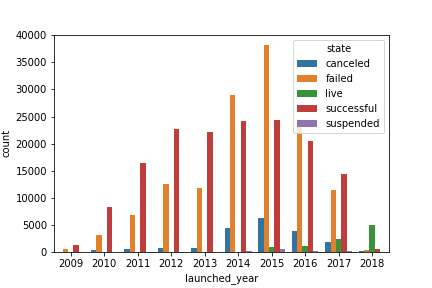
\includegraphics{plots/state_year.png}
\caption{Figure 1. Total number of projects by project status}
\end{figure}

While pledged amount is not included in the predictors as it is not
observable at the launch of the project,it's important to understand its
relationship with the project status and project goal. \emph{Figure 2}
illustrates that successful projects raised more while asked for less,
compared to failed projects.

\begin{figure}
\centering
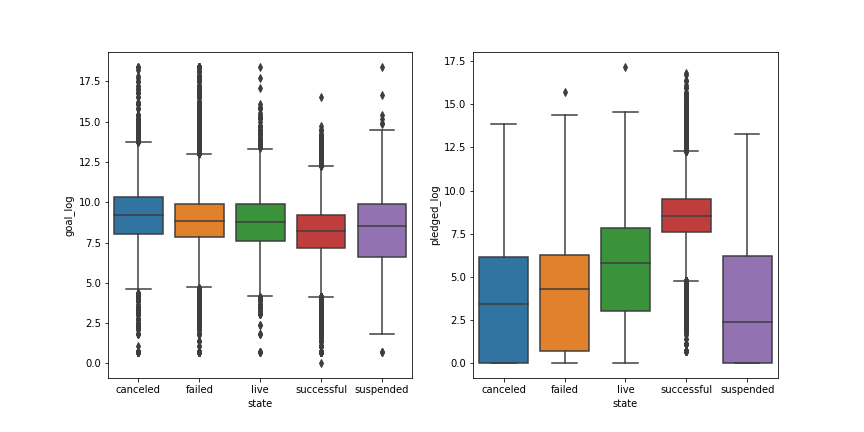
\includegraphics{plots/goal_status.png}
\caption{Figure 2. Goal and pledged amount by project status}
\end{figure}

Next I explored patterns of successful projects, whether the rate of
success varies by category, gender and location. The crosstab suggests
that projects with certain attributes tend to have higher rate of
success.

\emph{Figure 3} shows that projects launched in earlier years are more
likely to succeed on Kickstarter. This could have several explanations.
First, the platform is more competitive as Kickstarter become more
popular over the year. As shown in Figure one, the total number of
successful projects remained stable, but failed projects has steadily
increased. Second, early adoptors of the platform are usually enthuasits
of crowdsourcing and therefore, might be more serious about their
project quality, and make more effort to promote the campaign.

\begin{figure}
\centering
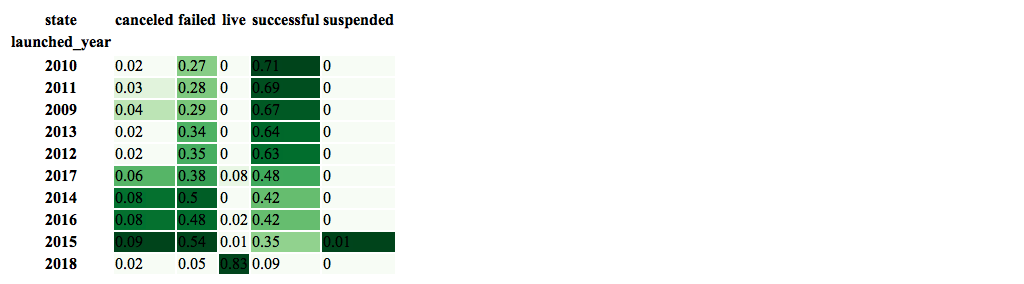
\includegraphics{plots/year_table.png}
\caption{Figure 3. Share of projects by project status each year}
\end{figure}

\emph{Figure 4} shows that on average, names perceived as female are
more likely to succeed. This is consistent with (Marom, Robb, and Sade
2016) that crowdfunding reduces the barriers of female entrepreneurs to
raise capital. The authors find that while female creators made up about
35\% of the project leaders, their rates of success are higher than male
creators, even after controlling for category and goal amount.

\begin{figure}
\centering
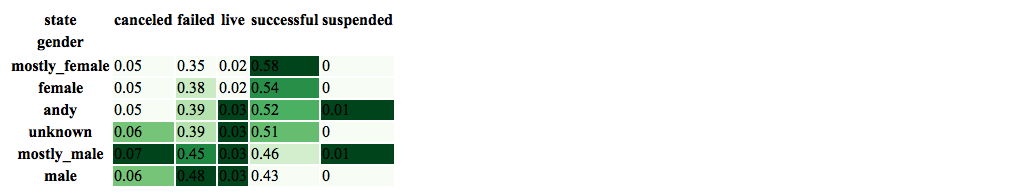
\includegraphics{plots/gender_table.png}
\caption{Figure 4. Share of projects by project status for type of
gender}
\end{figure}

The third table showed significant variance in successful rates for
different category of projects - dance, theatre, comics and design on
average have a successful rate over 60\% while fashion, journalism and
technology have a successful rate below 30\%.

\begin{figure}
\centering
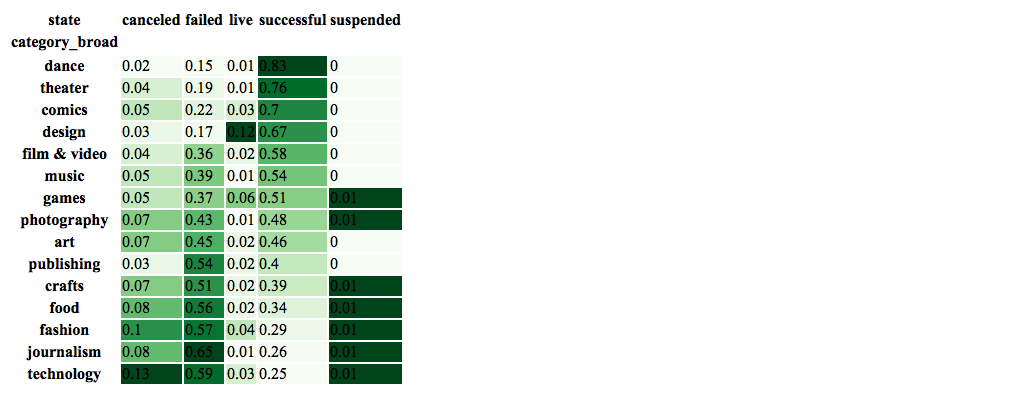
\includegraphics{plots/cat_table.png}
\caption{Figure 5. Share of projects by project status for each
category}
\end{figure}

\subsubsection{Algorithms and
Techniques}\label{algorithms-and-techniques}

This is a supervised learning problem, and the prediction is a binary
outcome, with successful projects coded as "1" and failed projects coded
as "0". The exploratory visualization also indicates that the underlying
relationship is rougly linear, so logistic algorithms would be suitable
for this question. The logit output can also be interpreted as a
probability, a nice feature to have for predicting the successful rate.

Two additional emsemble models are also utilized to compare the
performance:

\begin{enumerate}
\def\labelenumi{\arabic{enumi}.}
\tightlist
\item
  Random forest: good for both linear and non-linear models.
\item
  Boosted Tree: good for large feature sets and non-linear models
\end{enumerate}

Scaling and normalization techniques are applied to numerical variables
before fitting the models. Categorical variables are converted to
dummies using one-hot-encoding.

\subsubsection{Benchmark}\label{benchmark}

The naive predictor, in which we predict every campaign to be
successful, has an accuracy score of 0.5415, and an F-1 score of 0.5962.
This will serve as the main benchmark model to evaluate the model
performance.

Another benchmark model is a similar project from a per-reviewed study
\emph{(Greenberg et al. 2013)}. The author used data on all Kickstarter
projects that finished between: 6/18/2012 and 11/9/2012. The attributes
used as predictors are slightly different, summarized below:

\begin{enumerate}
\def\labelenumi{\arabic{enumi}.}
\tightlist
\item
  Goal in dollars of the project
\item
  Project category (eg. Music, or Dance, or Video Game)
\item
  Number of rewards available
\item
  Length of project in Days
\item
  Connected to twitter Boolean
\item
  Video present Boolean
\item
  Connected to Facebook Boolean
\item
  Number of facebook friends
\item
  Number of twitter followers
\item
  Sentiment (pos, neg, or neutral)
\item
  Number of sentences in project description
\item
  Outcome variable Boolean
\end{enumerate}

The authors evaluated the performance of radial basis, polynomial and
sigmoid kernel functions with varying costs for support vector machines.
The also tested decision tree models with AdaBoosting. The best
performing model were able to predict the success of a crowdfunding
project with 68\% accuracy.

\subsection{III. Methodology}\label{iii.-methodology}

\subsubsection{Data Preprocessing}\label{data-preprocessing}

One major component of the data processing is utilizing text analysis to
convert project title and descriptions to numeric values. For this task,
I use sentiment analysis from
\href{https://textblob.readthedocs.io/en/dev/}{TextBlob} package.
Polarity is float which lies in the range of {[}-1,1{]} where 1 means
positive statement and -1 means a negative statement. Subjective
sentences generally refer to personal opinion, emotion or judgment
whereas objective refers to factual information. Subjectivity is also a
float which lies in the range of {[}0,1{]}.

An example from the dataset is shown below:

\emph{Last year, I completed my first novel, The Circumstance of
Marriage. Now I need your help to get an editor to get it published!}

The assigned sentiment value is:

\emph{Sentiment(polarity=0.15625, subjectivity=0.19999999999999998)}

After text analysis, key steps to process the data are:

\begin{enumerate}
\def\labelenumi{\arabic{enumi}.}
\tightlist
\item
  \textbf{Duplicated projects}: the dataset is composed of data from 4
  independent crawls on 2015-12-17, 2016-06-15, 2017-02-15 and
  2018-02-15. Therefore, duplicated projects are checked and removed.
\item
  \textbf{Outliers}: A data point with a feature that is beyond an
  outlier step outside of the IQR (1.5 times) for that feature is
  considered abnormal. Observations with at least two abnormal features
  are removed from the analysis (1.4\% of the entire observations)
\item
  \textbf{Data normalization}: Log transformation is applied to all
  numeric varaibles to achieve a normalized distribution
\item
  \textbf{Data scaling}: although logistic models and decision trees are
  not affected by feature scaling, SVM and CNN are still susceptible.
  min-max scaler is applied to all nummeric variables.
\end{enumerate}

\subsubsection{Implementation}\label{implementation}

Three models were trained on the prepocesed training data (190,609
observations). Training time, accuracy score and F-1 score are stored to
compare the performance of different models.

Then I use GridSearch to search the optimal parameters to tune the
performance of Random Forest model. A list of tuning parameters is shown
below:

\begin{itemize}
\tightlist
\item
  \textbf{n\_estimators}: {[}10, 50, 100, 500{]}
\item
  \textbf{min\_samples\_split}: {[}2, 5, 10{]}
\item
  \textbf{min\_samples\_leaf}: {[}1, 5, 10{]}
\end{itemize}

This improved the accuracy score from 0.8018 to 0.8201, and F-1 score
from 0.8218 to 0.8247

Finally, I use feature importance to look for the features with most
predictive power in the model.

\subsubsection{Refinement}\label{refinement}

For the text analysis, I initially considered classifying the sentence
structure of the headline and use structure type as input. This involves
calculating pair-wise similarity matrix for each tokenized titles, and
then using K-means to find clusters. However, this approach failed to
identify meaningful types of sentence structures, and I decided to use
sentimental analysis instead.

For the training models, I also considered Support Vector Machine and
Conventional Neural Network. However, the training time for 190k
observations turns out to be computationally expensive.

\subsection{IV. Results}\label{iv.-results}

\subsubsection{Model Evaluation and
Validation}\label{model-evaluation-and-validation}

20\% of the dataset is held for testing. The model is trained on the
rest of the data, with 190,609 obseravations. Figure 6 shows the time
and score of three models for 1\%, 10\% and 100\% of the sample
respectively.

\begin{figure}
\centering
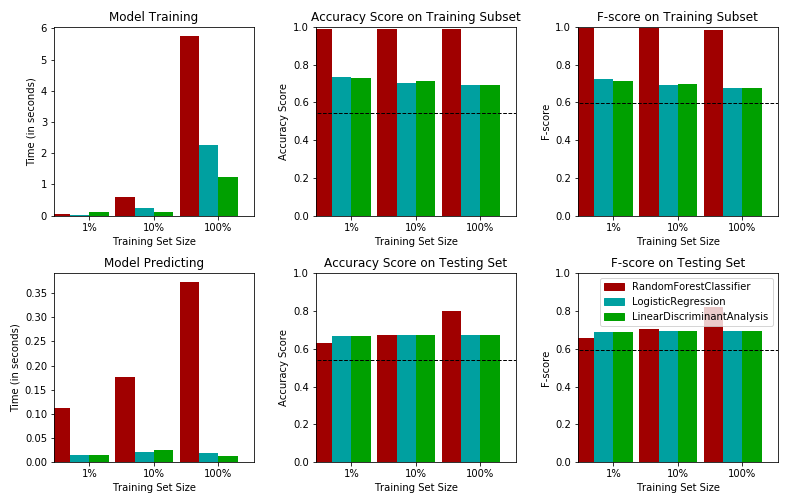
\includegraphics{plots/result.png}
\caption{Figure 6. Predicting time and accuracy score}
\end{figure}

I chose the RandomForest model as the final model because it has the
highest accuracy score on testing set, within a reasonable training
time.

\begin{figure}
\centering
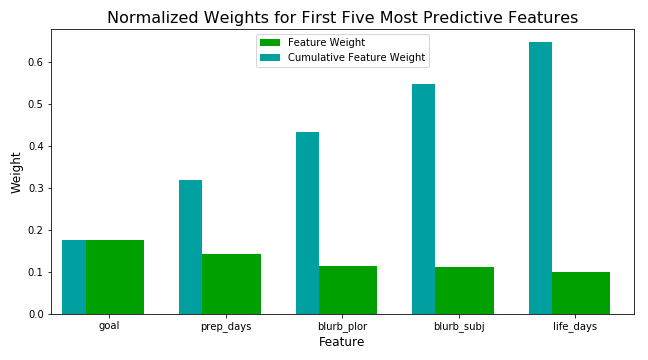
\includegraphics{plots/rf_imp.png}
\caption{Figure 7. Feature importance of Random Forest algorithm}
\end{figure}

The normalized weights for five most predictive features in the random
forests are Goal, Days spent on preparing for the campaign, Polarity of
the campaign description, Subjectivity of the campgain description and
lastly, Days to raise money.

\subsubsection{Justification}\label{justification}

All three models outperfom the accuracy score of the navie predictor
(accuracy score of 0.5415, and an F-1 score of 0.5962). The logistic
model achieved an accuracy score of 69\%, which is very similar to the
score published by the peer reviewed study.

Random forest outperforms other models when trained on full set by a
large margin.

\subsection{V. Conclusion}\label{v.-conclusion}

\subsubsection{Reflection}\label{reflection}

Overall, I think a 82\% accuracy rate meets the expectation of giving
people guidance on whether their chance of getting funded successfully.
Attributes that are most important to the change of success, namely
campaign goal and project description, are easy fix that people can
implement to increase their likelihood of success. How well this model
translates to other crowdsourcing sites such as Indiegogo however, is in
question as different sites might attract very different funders who may
have different preferences over certain attributes.

One issue I realized with the Random Forest model (or other machine
learning model) is that the method is designed to solve the problem of
prediction, not parameter estimation. However, if the model predicts a
low success rate of a campaign, it would be helpful to also indicate
what attributes are holding back the performance, and how to improve the
success rate. While Random Forest does produce featuer importance, it
lacks estimation of standard errors on the coefficients.

As an experiment, I applied Logistic Regression from the stats package
which gives parameter estimations on the same training set. The
regression result is shown below, and Figure 8 shows the coefficients of
each feature.

{[}Table 3. Regression results{]}

\begin{longtable}[]{@{}lllllll@{}}
\toprule
var & coef & std err & z & P\textgreater{} z & {[}0.025 &
0.975{]}\tabularnewline
\midrule
\endhead
goal & -6.2287 & 0.069 & -90.612 & 0.000 & -6.363 &
-6.094\tabularnewline
life\_days & -1.3034 & 0.053 & -24.362 & 0.000 & -1.408 &
-1.199\tabularnewline
prep\_days & 1.8486 & 0.026 & 71.725 & 0.000 & 1.798 &
1.899\tabularnewline
slug\_plor & 1.6692 & 0.126 & 13.203 & 0.000 & 1.421 &
1.917\tabularnewline
blurb\_plor & 1.4147 & 0.121 & 11.644 & 0.000 & 1.177 &
1.653\tabularnewline
blurb\_subj & -0.0235 & 0.017 & -1.362 & 0.173 & -0.057 &
0.010\tabularnewline
gender\_female & 0.3356 & 0.050 & 6.649 & 0.000 & 0.237 &
0.434\tabularnewline
gender\_male & -0.1434 & 0.050 & -2.893 & 0.004 & -0.241 &
-0.046\tabularnewline
gender\_mostly\_female & 0.4490 & 0.055 & 8.212 & 0.000 & 0.342 &
0.556\tabularnewline
gender\_mostly\_male & -0.0688 & 0.054 & -1.268 & 0.205 & -0.175 &
0.038\tabularnewline
gender\_unknown & 0.2531 & 0.050 & 5.064 & 0.000 & 0.155 &
0.351\tabularnewline
launch\_month\_2 & 0.1245 & 0.025 & 4.917 & 0.000 & 0.075 &
0.174\tabularnewline
launch\_month\_3 & 0.1706 & 0.025 & 6.881 & 0.000 & 0.122 &
0.219\tabularnewline
launch\_month\_4 & 0.0847 & 0.025 & 3.402 & 0.001 & 0.036 &
0.134\tabularnewline
launch\_month\_5 & 0.0757 & 0.025 & 3.068 & 0.002 & 0.027 &
0.124\tabularnewline
launch\_month\_6 & 0.0408 & 0.025 & 1.641 & 0.101 & -0.008 &
0.090\tabularnewline
launch\_month\_7 & -0.1587 & 0.024 & -6.528 & 0.000 & -0.206 &
-0.111\tabularnewline
launch\_month\_8 & -0.1098 & 0.025 & -4.431 & 0.000 & -0.158 &
-0.061\tabularnewline
launch\_month\_9 & 0.0656 & 0.025 & 2.615 & 0.009 & 0.016 &
0.115\tabularnewline
launch\_month\_10 & 0.1270 & 0.025 & 5.134 & 0.000 & 0.078 &
0.175\tabularnewline
launch\_month\_11 & 0.1004 & 0.025 & 3.986 & 0.000 & 0.051 &
0.150\tabularnewline
launch\_month\_12 & -0.0517 & 0.028 & -1.876 & 0.061 & -0.106 &
0.002\tabularnewline
category\_broad\_comics & 1.2398 & 0.035 & 35.788 & 0.000 & 1.172 &
1.308\tabularnewline
category\_broad\_crafts & -0.4674 & 0.038 & -12.316 & 0.000 & -0.542 &
-0.393\tabularnewline
category\_broad\_dance & 1.9088 & 0.054 & 35.618 & 0.000 & 1.804 &
2.014\tabularnewline
category\_broad\_design & 1.6045 & 0.034 & 47.021 & 0.000 & 1.538 &
1.671\tabularnewline
category\_broad\_fashion & -0.7141 & 0.029 & -24.605 & 0.000 & -0.771 &
-0.657\tabularnewline
category\_broad\_film \& video & 0.8775 & 0.021 & 41.897 & 0.000 & 0.836
& 0.919\tabularnewline
category\_broad\_food & -0.1135 & 0.026 & -4.339 & 0.000 & -0.165 &
-0.062\tabularnewline
category\_broad\_games & 0.6375 & 0.026 & 24.880 & 0.000 & 0.587 &
0.688\tabularnewline
category\_broad\_journalism & -0.7694 & 0.045 & -16.971 & 0.000 & -0.858
& -0.681\tabularnewline
category\_broad\_music & 0.4412 & 0.021 & 21.500 & 0.000 & 0.401 &
0.481\tabularnewline
category\_broad\_photography & 0.3203 & 0.035 & 9.179 & 0.000 & 0.252 &
0.389\tabularnewline
category\_broad\_publishing & -0.2539 & 0.022 & -11.777 & 0.000 & -0.296
& -0.212\tabularnewline
category\_broad\_technology & -0.4170 & 0.026 & -16.310 & 0.000 & -0.467
& -0.367\tabularnewline
category\_broad\_theater & 1.6380 & 0.036 & 45.054 & 0.000 & 1.567 &
1.709\tabularnewline
\bottomrule
\end{longtable}

\begin{figure}
\centering
\includegraphics{plots/lg_params.png}
\caption{Figure 8. Logistic regression coefficients}
\end{figure}

This show the magnitude as well as the direction of each parameters: if
you want to improve your rate of success, you should consider a smaller
goal, go for a shorter fundraising timeframe, spend more time preparing
for the campaign, and make sure your project description is both
positive and subjective.

\subsubsection{Improvement}\label{improvement}

There are a couple areas to improve this project:

\begin{enumerate}
\def\labelenumi{\arabic{enumi}.}
\item
  Image analysis: another potential attribute to include would be the
  characterstics of creator's profile image: would presenting a human
  face increase the chance of getting funded? Does the hue of the image
  matter? This however, requires significant storage and computing power
  to implement using Conventional Neural Network.
\item
  Feature selection: PCA is not recommended for datasets containing a
  mix of continuous and categorical variables. Research has suggested
  using multiple correspondence analysis for mixed data types. I need
  more understandings of the techniques before implementing it.
\item
  Sentiment analysis: Ideally I want to train the sentiment analysis
  classifier on the Kickstarter dataset, which would be more relevant.
\end{enumerate}

\section{Reference}\label{reference}

\begin{itemize}
\tightlist
\item
  Greenberg, Michael, Bryan Pardo, Karthic Hariharan, and Elizabeth
  Gerber. 2013. ``Crowdfunding Support Tools: Predicting Success \&
  Failure.'' In , 1815--20. doi:10.1145/2468356.2468682.
\item
  Marom, Dan, Alicia Robb, and Orly Sade. 2016. ``Gender Dynamics in
  Crowdfunding (Kickstarter): Evidence on Entrepreneurs, Investors,
  Deals and Taste-Based Discrimination.''
\item
  Mollick, Ethan R., and Venkat Kuppuswamy. 2014. ``After the Campaign:
  Outcomes of Crowdfunding.''
\end{itemize}


    % Add a bibliography block to the postdoc
    
    
    
    \end{document}
